\documentclass[a4paper,11pt,fleqn]{article}

\usepackage[brazil]{babel}
\usepackage[utf8]{inputenc}
\usepackage{xspace}
\usepackage{color}
\usepackage{graphicx}
\usepackage{hyperref}
\usepackage{enumitem}



\newcommand{\blue}[1]{\textcolor{blue}{#1}}

\title{Projeto Final\\
Programação Orientada a Objetos - MC302}
\author{Alunos: André Papoti, Bruno Falkenburg, Lucas Ramos, \\
Nicolas França, Sophia Estrêla\\\\
Professora: Esther Colombini\\\\
Unicamp - Instituto de Computação\\}
\date{Junho de 2018}

\begin{document}

\maketitle

\begin{abstract}
\noindent

A intenção do projeto é ser um sistema interno de uma imobiliária, ou seja, é feito considerando os corretores como usuários e a imobiliária em sí como o administrador (root). Esses usuários gerenciam imóveis, clientes, proprietários e propostas e o adiministrador gerencia os corretores.

É importante destacar que o usuário final são os corretores e outros possíveis funcionários da imobiliária (que é o caso do nosso administrador).

Queremos fazer buscas de imoveis do melhor agrado do cliente, assim como servir como um banco de dados afim de armazenar os dados do cliente e do proprietário em sí.

Queremos enfatizar que o projeto não foi pensado para acesso direto de terceiros, como compradores e proprietários, pois a nossa regra de negócio diz que esses dados são sigilosos.

Agora em sua etapa final o sistema da sugestões de imóveis do agrado do cliente, cruzando suas preferências com os imóveis disponíveis.

O sistema foi pensado consultando uma corretora real, de forma que este se adapte as necessidades de um usuário do mundo real. Este também trará o benefício de tornar processos do dia-a-dia de uma imobiliaria, como a oficialização de uma proposta se tornar mais fácil e ágil.

\end{abstract}

\section{Funcionalidades}
\label{s:funcionalidades}

\subsection{Funcionalidades Implementadas}
\label{ss:func-impl}


Foram implementadas as seguintes funcionalidades nesta etapa do projeto:

\begin{enumerate}
    \item Adição de novos Corretores pelo Administrador;
    \item Adição de novos Imoveis;
    \item Adição de novos Corretores
    \item Adição de novos Clientes;
    \item Adição de Propostas;
    \item Adição de Proprietários dos imóveis;
    \item Remoção de Corretores pelo Administrador;
    \item Remoção de Imoveis;
    \item Remoção de Corretores
    \item Remoção de Clientes;
    \item Finalização de Propostas: propostas pode estar ativas ou não;
    \item Listagem dos Corretores pelo Adiministrador;
    \item Listagem dos Imoveis relacionados as preferencias de um cliente;
    \item Listagem das Propostas cujo o Corretor foi intermediário;
    \item Listagem dos Clientes cujo responsável é o Corretor;
    \item Listagem dos Proprietarios de todos os Imoveis disponíveis no sistema;
    \item Salvar dados no banco de dados;
\end{enumerate}

\section{Ferramentas Utilizadas}
\label{s:ferramentas}

\subsection{PostgreSQL}
\label{ss:postgre}

PostgreSQL é um SGBD (Sistema Gerenciador de Banco de Dados) objeto-relacional. Isso significa que os dados no banco são modelados como entidades relacionadas, semelhantes
 a tabelas, acrescidos de estruturas típicas de orientação a objetos. A linguagem utilizada no PostgreSQL é a SQL.

 Foi utilizado para criação e gerenciamento de um banco de dados que armazenará os dados referentes às entidades do sistema.

 Nós precisamos criar um Diagrama de Entidade e Relacionamento baseado no nosso Diagrama UML. Já ter o UML de antemão nos ajudou bastante, mas ainda assim foi
bastante desafiante a criação desse DER, pois tivemos que fazer um mapeamento de PK (Primary Key: Chave Primária) e FK (Foregin Key: Chave Estrangeira) que durante
o tempo passou a dar bastante dor de cabeça. A vantagem de tudo isso foi a experiência que ganhamos em tão pouco tempo.

 O código sql esta no arquivo sqlAtual.sql, usando a versão 9.6 do PostgreSQL.

\begin{enumerate}
    \item\texttt{apartamentos}
    \item\texttt{casas}
    \item\texttt{cliente\_formas\_pagamento}
    \item\texttt{clientes}
    \item\texttt{condominio\_lazeres}
    \item\texttt{condominios}
    \item\texttt{corretores}
    \item\texttt{enderecos}
    \item\texttt{formas\_pagamento}
    \item\texttt{gerentes}
    \item\texttt{imoveis}
    \item\texttt{imoveis\_construidos}
    \item\texttt{imovel\_formas\_pagamento}
    \item\texttt{imovel\_restricoes}
    \item\texttt{lazeres}
    \item\texttt{pagamentos}
    \item\texttt{pessoas}
    \item\texttt{preferencias}
    \item\texttt{preferencias\_construcao}
    \item\texttt{propostas}
    \item\texttt{proprietarios}
    \item\texttt{restricoes}
    \item\texttt{terrenos}
    \item\texttt{tipos\_imovel}
\end{enumerate}

\begin{figure}[h!]
  \begin{center}
    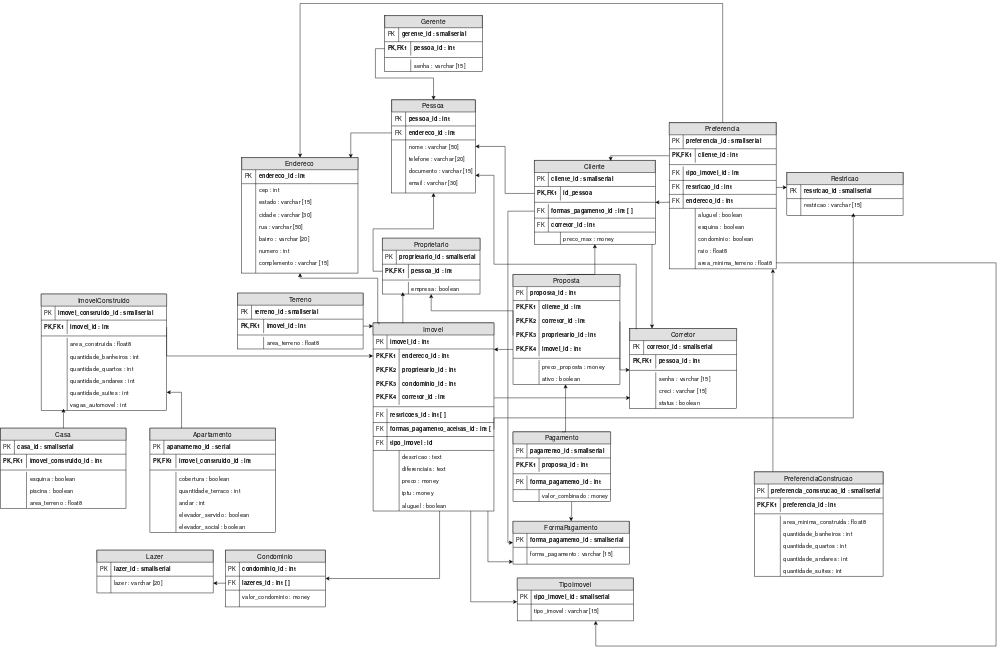
\includegraphics[scale=0.4]{imagens/der.png}
  \end{center}
  \caption{Como foi projetado o nosso Diagrama de Entidades e Relacionamentos (DER)}
  \label{f:trello}
\end{figure}


\subsection{Git e GitHub}
\label{ss:github}

O GitHub é uma plataforma que permite hospedar e compartilhar arquivos, com foco em arquivos de código-fonte.

Por utilizar o Git para controle de versão, os programadores podem trabalhar em ramificações locais do projeto e enviar ao repositório hospedado no GitHub os arquivos
 que trabalharam, registrando todas alterações e permitindo que outro desenvolvedor que esteja trabalhando no projeto possa permanecer atualizado sobre o progresso
  do outro.

Por conta dos benefícios que esta plataforma traz, o grupo está utilizando para controle do código - garantindo que todos estejam com versões atualizadas
 e possam com a mesma facilidade revisar e alterar o próprio código ou o de outro membro da equipe - e dos demais arquivos relacionados ao projeto. 

\subsection{Trello}
\label{ss:trello}

O Trello é o nosso organizador de projetos. Com ele temos um board, que tem um conjunto de listas. E cada lista tem é um conjunto de card.
  Como usamos o método Kanban, os cards transitam entre lists até chegar a lista "Conclusão".

A estrutura do nosso board pode ser vista na Figura~\ref{f:trello}.

\begin{figure}[h!]
  \begin{center}
    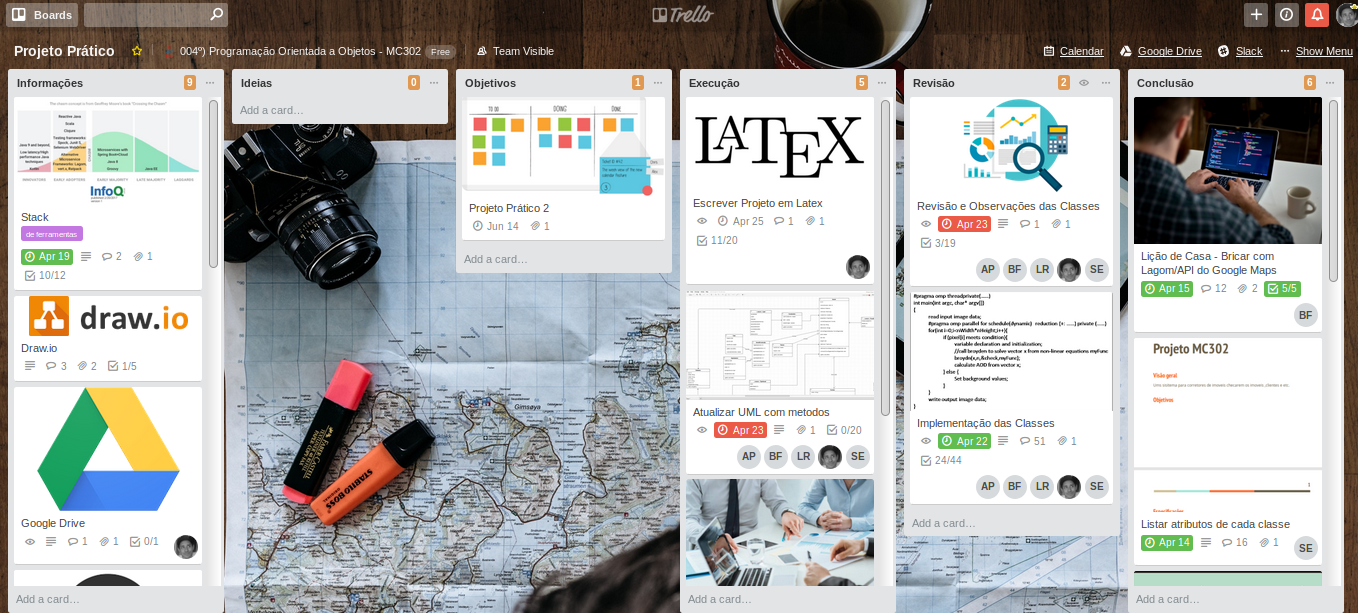
\includegraphics[scale=0.3]{imagens/trello.png}
  \end{center}
  \caption{Como o Trello é usado no nosso projeto}
  \label{f:trello}
\end{figure}

O nosso board é dividido em 6 listas: Informações, Ideias, Objetivos, Execução, Revisão e Conclusão.

Informações: Tem cards com informações gerais, links, recursos e descrições e documentações das ferramentas que estamos utilizando.

Ideias: Lista para cards de ideias gerais.

Objetivos: Lista com os objetivos futuros que estamos galgando.

Execução: Lista com as tarefas que estão sendo executadas naquela fase do projeto.

Revisão: Revisão das tarefas terminadas em Execução.

Conclusão: Tarefas que foram em grande parte feitas.

\subsection{Google Hangouts}
\label{ss:google-hangouts}

O Google Hangouts é o serviço padrão da Google para comunicação em tempo real.
  Usamos muito durante nossas reuniões remotas. Normalmente nos encontramos mais online
    do que fisicamente devido aos diferentes horários em comum entre os membros.

Conseguimos com ele compartilhamento de tela compartilhamento de áudio e essas features são as mais usadas entre
  nós.

\subsection{Google Drive}
\label{ss:google-drive}

Usamos para ter os dados mais atualizados possível de forma sincronizada. O Trello e o draw.io tem integração com o Drive que
  usamos constantemente entre nós.

\subsection{draw.io}
\label{ss:draw}

Para a criação do Diagrama de Classes UML presente neste arquivo foi utilizado o draw.io, uma ferramenta online de criação e edição de diversos tipo de diagramas.
 O site permite integração dos diagramas com o Google Drive, que é útil para compartilhamento dos diagramas e edição simultânea por mais de um membro.


\subsection{Whatsapp}
\label{ss:whatsapp}

Usado para comunicação rápida entre os membros.

\subsection{LaTeX}
\label{ss:latex}

O \LaTeX é utilizado para a formatação do nosso relatório final sobre o projeto. O arquivo lido atualmente foi compilado pelo LaTeX e
  nos proporciona vários benefícios relacionados a escrita. É uma ferramenta com grande uso pela comunidade acadêmica.

\subsection{WindowsBuilder}
\label{ss:windows-builder}

O WindowsBuilder é um plugin para Eclipse para facilitar a criação de interfaces gráficas (GUI). Nessa fase do projeto essa
  ferramenta vai nos ajudar a entregar parte de um conjunto de interfaces gráficas simples. 




\end{document}
